\documentclass{article}

%%% packages %%%%%%%%%%%%%%%%%%%%%%%%%%%%%%%%%%%%%%%%%%%%%%%%

%-- page setup ----------------------------------------------

\usepackage[utf8]{inputenc}
\usepackage[a4paper, margin=1in]{geometry}

%-- font ----------------------------------------------------

\usepackage[T1]{fontenc}

%-- img ---------------------------------------------------------

\usepackage{graphicx}

%-- head/foot -----------------------------------------------

\usepackage{fancyhdr}

\pagestyle{fancy}

\fancyhead[l]{Vincent von Schmidt\\Niklas Zock}
\fancyhead[c]{L17 - Informatik}
\fancyhead[R]{\today}

\renewcommand{\footrulewidth}{0.4pt}
\fancyfoot{}
\fancyfoot[L]{Software - Projekt\\Mini Chess}
\fancyfoot[R]{\thepage}

%------------------------------------------------------------
%%%%%%%%%%%%%%%%%%%%%%%%%%%%%%%%%%%%%%%%%%%%%%%%%%%%%%%%%%%%%

\title{\textbf{Software - Projekt\\Mini Chess}}
\date{\vspace{-5ex}}

\begin{document}

\maketitle
\thispagestyle{fancy}

%%% content %%%%%%%%%%%%%%%%%%%%%%%%%%%%%%%%%%%%%%%%%%%%%%%%%

\tableofcontents
\newpage

%------------------------------------------------------------

\section{Ziele}\label{section-goals}

\subsection{Minimalanforderung}
\begin{itemize}
    \item simple Oberfläche $\rightarrow$ Spielfläche, Start / Resign Button
    \item rating algo $\rightarrow$ Player vs. CPU
    \item 3x3
    \item pygame GUI
\end{itemize}

\subsection{Zusatzanforderung}
\begin{itemize}
    \item 4x4; 5x5
    \item Player vs. Player
    \item PyQt with embeded pygame $\rightarrow$ clean GUI
    \item Multithreading
\end{itemize}

%------------------------------------------------------------

\newpage
\section{Systemanforderung}\label{section-requirements}

\subsection{Hardware}
\begin{itemize}
    \item 8 GB RAM
    \item 32 MB Speicher
    \item Multicore CPU
    \item Maus und Tastatur
    \item Farbbildschirm (empfohlen)
\end{itemize}

\subsection{Software}
\begin{enumerate}
    \item Ausführen via .exe $\rightarrow$ Windows 10 21H2 +
    \item Ausführen via Python
        \begin{itemize}
            \item Python 3.11+ $\rightarrow$ Python 3.11 für bessere Effizents
            \item Python libarys $\rightarrow$ einfacher Installationsprozess via requirements.txt
                \begin{itemize}
                    \item PyQt6
                    \item pygame 2.4
                \end{itemize}
        \end{itemize}
\end{enumerate}

\subsection{Merkmale}
sehr großer Fokus: $++$    großer Fokus: $+$    mittlerer Fokus: $o$    kleiner Fokus: $-$    sehr kleiner Fokus: $--$
\begin{center}
    \begin{tabular}{ |c|c| }
        \hline
        Merkmale & Gewichtung \\
        \hline
        Benutzerfreundlichkeit & $++$ \\
        \hline
        Korrektheit & $+$ \\
        \hline
        Wartungsfreundlichkeit & $+$ \\
        \hline
        Zuverlässigkeit & $++$ \\
        \hline
        Effizienz & $o$ \\
        \hline
    \end{tabular}
\end{center}


%------------------------------------------------------------

\newpage
\section{Produktumgebung}\label{section-product}

\subsection{Benutzeroberfläche}

\subsubsection{Minimalanforderung}

\textbf{Startscreen:}
\begin{figure}[h]
    \centering
    \fbox{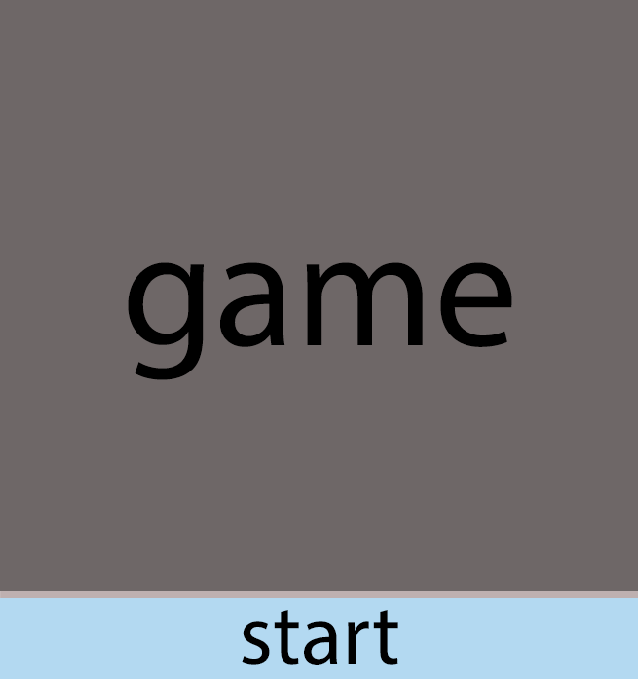
\includegraphics[width=3in, keepaspectratio]{img/min_start.png}}
\end{figure}

\textbf{Gamescreen:}
\begin{figure}[h]
    \centering
    \fbox{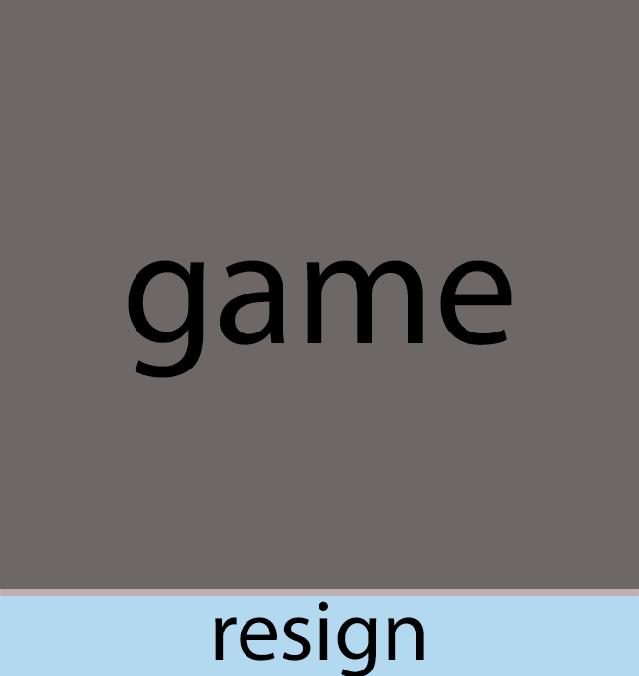
\includegraphics[width=3in, keepaspectratio]{img/min_game.png}}
\end{figure}

\newpage

\subsubsection{Zusatzanforderung}

\textbf{Startscreen:}
\begin{figure}[h]
    \centering
    \fbox{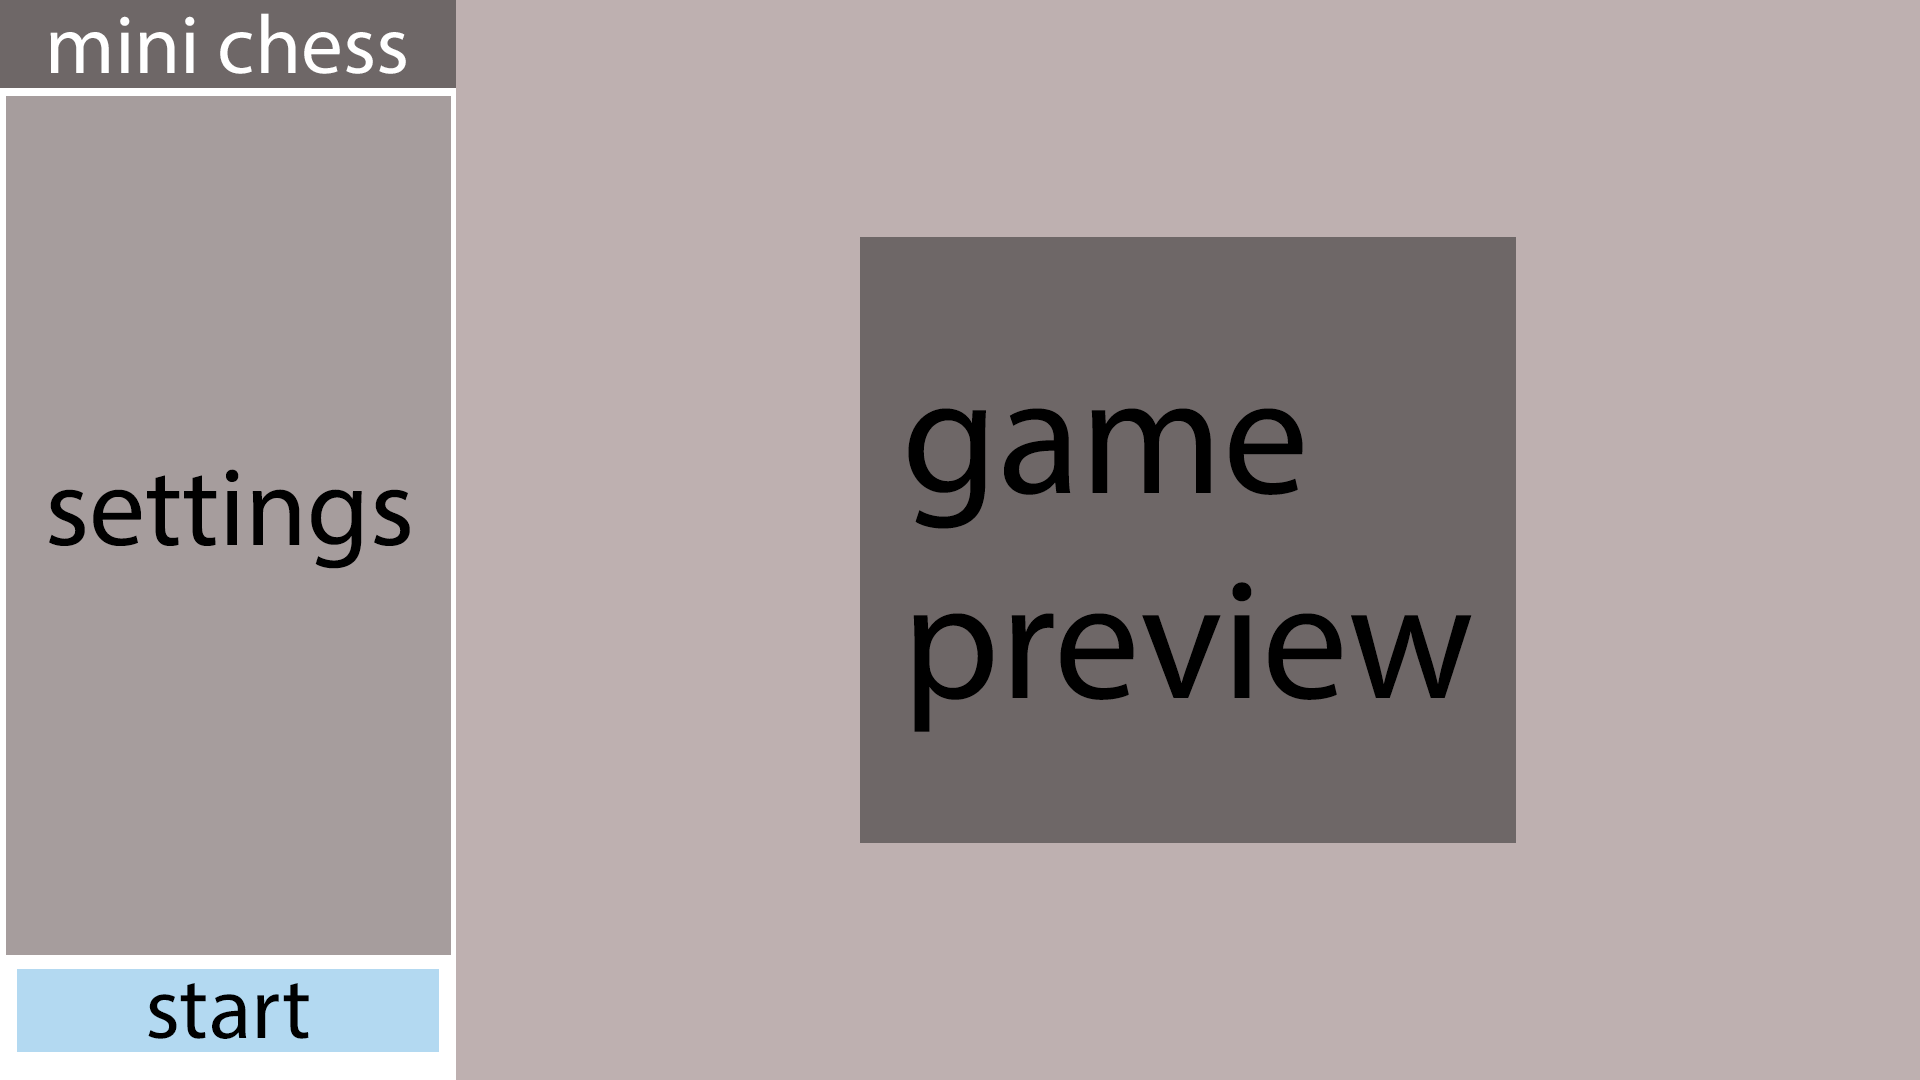
\includegraphics[width=\textwidth, keepaspectratio]{img/plus_start.png}}
\end{figure}

\textbf{Gamescreen:}
\begin{figure}[h]
    \centering
    \fbox{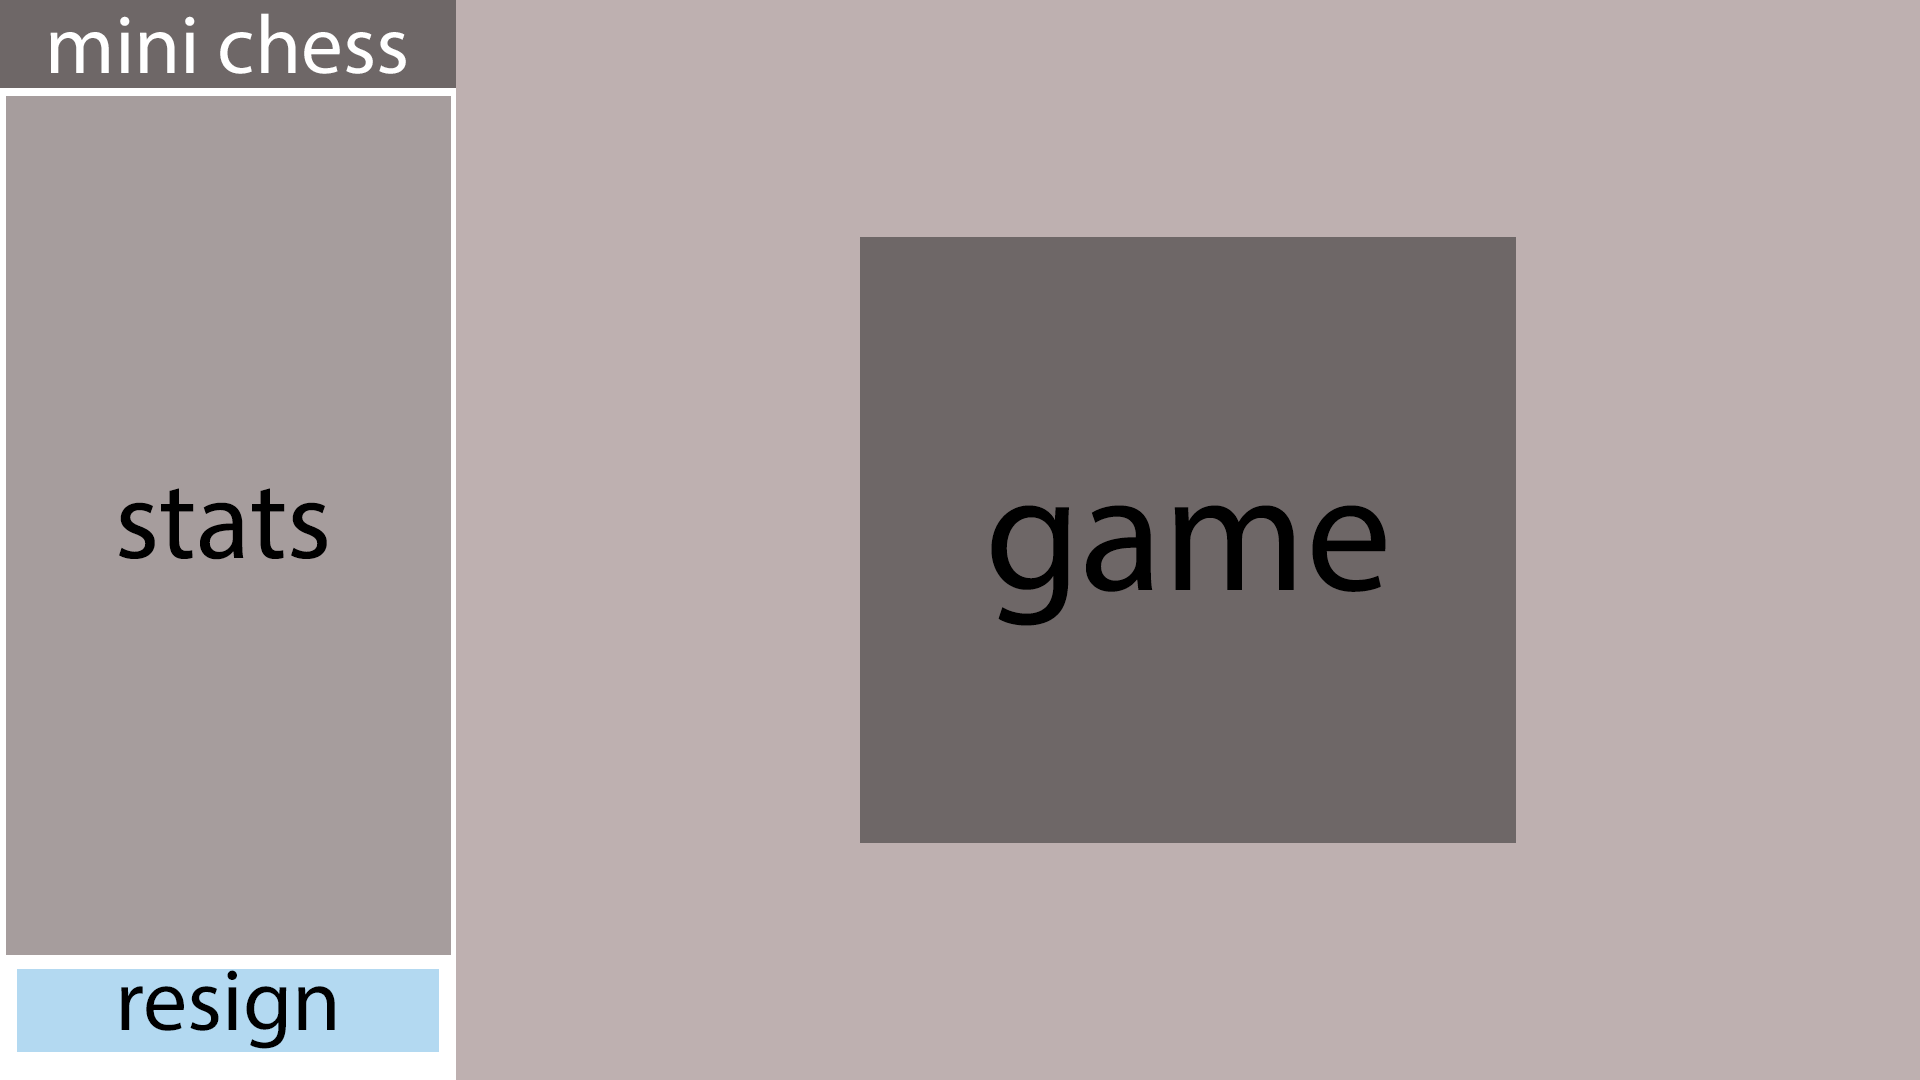
\includegraphics[width=\textwidth, keepaspectratio]{img/plus_game.png}}
\end{figure}

\newpage

\subsection{Klasendiagramm}

\subsubsection{Minimalanforderung}
ohne AI
\begin{figure}[h]
    \centering
    \fbox{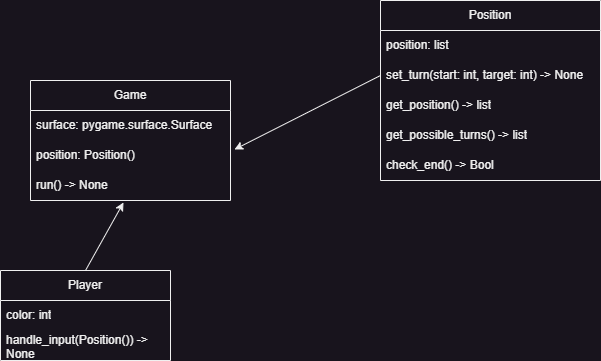
\includegraphics[width=4in,
    keepaspectratio]{img/class_diagramm_without_ai.png}}
\end{figure}

\subsubsection{Zusatzanforderung}
mit AI
\begin{figure}[h]
    \centering
    \fbox{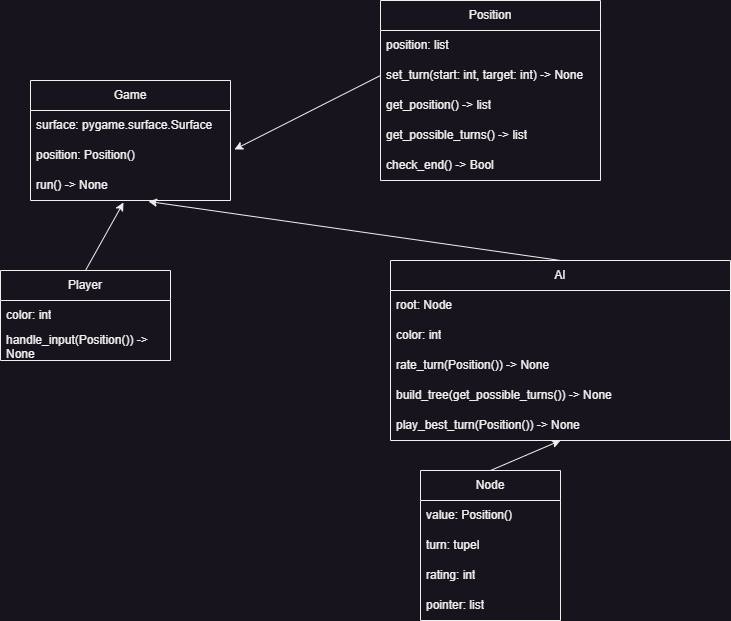
\includegraphics[width=4in, keepaspectratio]{img/class_diagramm_ai.png}}
\end{figure}

\newpage

\subsection{Spezifikationen}

\subsubsection{Game}

\textbf{run():} Beherbergt die main game loop, die den Spielzyklus ausführt, die GUI baut und das Spiel beendet.

\subsubsection{Position}

\textbf{set\_turn(start: int, target: int):} Bekommt den Zug als Integer der Felder. Führt den Zug aus und updated den Spielzustand. \\
\textbf{get\_position():} Gibt das Spielfeld als Liste zurück. \\
\textbf{get\_possible\_turns():} Gibt alle Möglichen Züge als Liste zurück. \\
\textbf{check\_end():} Gibt True zurück, wenn jemand gewonnen hat und merkt sich den Gewinner. \\

\subsubsection{Player}

\textbf{handle\_input(Position):}Bekommt die aktuelle Position. Kann dem Spieler die möglichen Züge anzeigen, Wartet auf einen Input des Spielers, überprüft ob dieser valide
ist und verarbeitet diesen. \\

\subsubsection{AI}
\textbf{rate\_turn(Position):} Bewertungsfunktion für die angegebene Position. \\
\textbf{build\_tree():} Lässt alle möglichen Züge bewerten und baut dann den Baum. \\
Zusatz: abschneiden \\
\textbf{play best turn():} Nimmt den besten Zug aus dem Baum und führt ihn aus. \\

\subsubsection{Node}
\textbf{Knoten des Baumes, die alle Informationen über den Zug speichern}

%------------------------------------------------------------

\newpage
\section{Arbeitstagebuch}\label{section-diary}

\subsection{Chronologie}
\subsection{Testläufe}

%------------------------------------------------------------

%%%%%%%%%%%%%%%%%%%%%%%%%%%%%%%%%%%%%%%%%%%%%%%%%%%%%%%%%%%%%

\end{document}
